\chapter{Definition der Use-Cases} \label{Umsetzung der Use-Cases und Evaluation}

\section{Kundenumfeld und typische Bedürfnisse} \label{Kundenumfeld und typische Bedürfnisse}

%kleine und mittlere Deployments... statt KMU. Bachelor-Arbeit war moving target
%Mein Ansatz: bis zu einer technischen Größenordnung ist das okay... Ansonsten Direct Connect oder Express Route
%Für kleine und mittlere Deployments (nicht KMU) -> keine kaufmännische sondern technologische Betrachtung
%Weniger Ebenen!

"Qualitätssicherung": Warum haben sich die Erkenntnisse aus dem Proposal zur Arbeit geändert? Halbe Seit
Wie bereits eingangs erwähnt, sollen die Use-Cases typische Bedürfnisse von Unternehmen aus dem kleinen und mittelständischen Bereich widerspiegeln (KMU). So ist die Grundannahme, dass der Kunde bereits Rechenressourcen in Selbstverwaltung (\glqq Private Cloud\grqq{}) besitzt. Weiterhin hat die Integration von Public Cloud-Diensten noch gar nicht oder nur oberflächlich stattgefunden: Es wurden ein paar Maschinen hochgefahren und bestimmte Internetdienste installiert. Über eine tiefergehende Koppelung mit bestehenden Diensten und Systemen hat der Kunde bisher keine Überlegungen angestellt. %Eine private Adressierung der Systeme ist noch nicht möglich, die Maschinen werden über die öffentlichen IPs aus dem Internet erreicht. Die Firma besitzt eine private Cloud
%ToDo: Genauer beschreiben, was beim Kunden schon zur Verfügung steht (Private Cloud) und dass das abstrahiert (vereinfacht) dargestellt wird


\section{Use Case 1: Basis Deployment}


Es wird ein Basis Deployment benötigt, um eine grundlegende Integration in die Firmeninfrastruktur zu ermöglichen.
%ToDo: Initial erwähnen, dass Amazon Web Services -> AWS, Microsoft Azure -> Azure
Der Fokus dieser Arbeit liegt auf den Public Cloud-Plattformen AWS und Azure sowie einer vereinfacht dargestellten Private Cloud. Die Annahme ist, dass diese bereits zur Verfügung steht und eine Menge an Diensten und Maschinen bereitstellt, die vom Kunden in Selbstverwaltung administriert wird.\\
Eine Hybrid Cloud besteht, wie bereits beschrieben, aus Public und Private Cloud. Da mit beiden Public Clouds getestet werden soll, wäre hier bereits eine Fallunterscheidung notwendig: Private Cloud <-> Azure bzw. Private Cloud <-> AWS. Um sich diese Fallunterscheidung sparen zu können, soll ein Dreieck ausgerollt werden, bei dem jeder Punkt eine Cloud-Plattform darstellt.
%Weitere Vorteile ergeben sich später: Redundanz, einfaches Skalieren _zwischen_ Public Clouds
%Bild Basis Deployment
Optimalerweise wird durch dieses Deployment auch die Redundanz erhöht: Fällt eine Verbindung aus bspw. zwischen AWS und Azure, so können Datenpakete weiterhin über die Private Cloud geroutet werden.
%Bild Link Fail

%Kein NAT -> Ende-zu-Ende-Kommunikation _aller_ Teilnehmer

Der Use-Case soll als Grundaufbau für alle weiteren Use-Cases dienen. Das Dreieck aus AWS, Azure und Private Cloud wird fortan als \textit{Backbone} bezeichnet.

\subsection{Vorauswahl geeigneter technischer Komponenten}
%PFS, AES Best Practices referenzieren
AWS und Azure bieten auf ihren Plattformen Unterstützung für Route-Based IPSEC-Tunnel. Darüber kann eine virtuelle Punkt-zu-Punkt (vgl. technische Grundlagen) hergestellt werden. Gleichzeitig werden übertragene Daten verschlüsselt und dadurch Integrität und Vertraulichkeit geschützt.\\
Weiterhin kann innerhalb der Tunnel BGP gesprochen werden, um ein dynamisches Routing zu ermöglichen \cite[S. 19]{AlShawi2020} \cite[S. 74-79]{Toroman2019}. Das dynamische Routing bietet den Vorteil, dass IPv4-Routen nicht manuell bei allen Gateways des Netzwerks bekannt gemacht werden müssen: Sobald ein Teilnehmer eine neue Route besitzt, wird dies via BGP den restlichen Teilnehmern bekannt gegeben.\\
%In technischen Grundlagen erwähnen: IaC, Provider, Module
%Mozilla Public License v2.0[2]
%Beispiel aus der Realität nennen: Switch - Kabel - Server
Für das automatisierte Deployment der Infrastruktur eignet sich Terraform der Firma Hashicorp. Es besitzt eine Vielzahl an \textit{Resources}, welche es ermöglichen, Infrastrukturkomponenten \texit{reproduzierbar} zu deployen. Im Gegensatz zu anderen Automatisierungsframeworks wie Ansible werden durch die implizite Referenzierung zwischen Ressourcen Infrastruktur-Abhängigkeiten aufgelöst.
Die Reihenfolge von Resource-Aufrufen innerhalb der Terraform-Module spielt keine Reihenfolge. So lassen sich komplexere Infrastrukturen installieren, ohne die Abhängigkeiten manuell auflösen zu müssen. Ressourcen, die keine Abhängigkeiten zueinander haben, werden parallel installiert.

%Todo: RFC 5737 in Einleitung (Documentation IPs)
\begin{lstlisting}[label=terraform-implicit-dependeny,caption=Durch die implizite Referenz auf \textit{aws\_vpc.example\_vpc.id} wird zuerst die Ressource \textit{example\_vpc} ausgeführt]
resource "aws_vpn_gateway" "example_gateway" {
	vpc_id = aws_vpc.example_vpc.id
}

resource "aws_vpc" "example_vpc" {
	cidr_block = "192.0.2.0/24"
	instance_tenancy = "default"
}
\end{lstlisting}

%PHPIPAM: GPLv3, Terraform Provider: Apache License 2.0
%https://web.archive.org/web/20201122173813/https://github.com/lord-kyron/terraform-provider-phpipam
%https://github.com/phpipam/phpipam
%https://web.archive.org/web/20201108102250/https://phpipam.net/
%https://blog.vyos.io/vyos-rolling-release-has-got-an-http-api
%https://web.archive.org/web/20210405210638/https://docs.vyos.io/en/latest/automation/vyos-api.html

Darüber hinaus wird ein IPAM benötigt zur IPv4-Adressverwaltung. Die automatische Zuteilung von Adressbereichen darf nicht dazu führen, dass Adressbereiche mehrfach verteilt werden oder sich Adressbereiche überlappen. Gewählt wurde hier das Werkzeug PHPIPAM: Es lässt sich sehr gut mit Terraform integrieren, da ein entsprechender Provider zur Verfügung steht.\\
Die VPN-Gateways, die das Backbone aufspannen, sind mit \textit{Virtual private gateway} bei AWS und \textit{VPN Gateway} bei Azure gesetzt. Dies sind die typischen \textit{Building-Blocks}, die von den Herstellern für VPN-Verbindungen angeboten werden. Nur wenn sich im Laufe der Arbeit herausstellen sollte, dass diese Systeme nicht interoperabel arbeiten, wird versucht, Alternativen zu finden. Als Router, der die Private Cloud repräsentiert, wurde ein VyOS Router gewählt. Dieser steht als Open Source zur Verfügung, es gibt allerdings auch bezahlten Support für Produktionsumgebungen. Der Router hat IPSEC- und BGP-Unterstützung und besitzt ein Command Line Interface, welches sich für das automatisierte Deployment mit Terraform als sehr vorteilhaft erweist, obwohl bisher kein Terraform Provider zur Verfügung steht (vgl. später). Eine REST-API steht ebenso zur Verfügung, aber diese ist zum Stand der Bachelor-Arbeit \textit{bleeding edge} und bisher eher dürftig dokumentiert. Die Annahme ist, dass der Router und das IPAM in der Private Cloud bereits vorhanden sind. Diese Komponenten sind nicht Teil des (Terraform-)Deployments.\\
Prinzipiell lassen sich viele Router-Modelle nutzen, insofern die Unterstützung für genannte Techniken vorhanden ist, bspw. CSR 1000V der Firma Cisco \cite{Durai2016}. Der offene VyOS Router bietet den Vorteil, dass keine Lizenzen für die Nutzung hinterlegt werden müssen, was in vielen Fällen manuelle Konfigurationen erfordert. Außerdem hätten passende Lizenzen beschafft werden müssen, was u.U. zu Verzögerungen der Bachelor-Arbeit geführt hätte.

\begin{figure}[h]
  \centering
  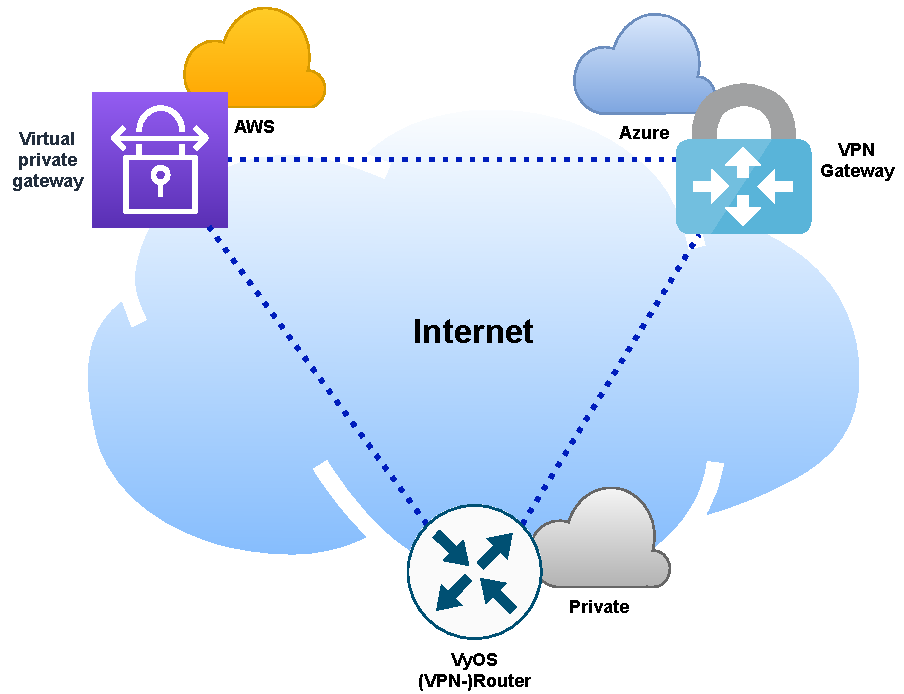
\includegraphics{Figures/Use-Case-1_Basis_Deployment.pdf}
  \caption{Basis Deployment}
  \label{grafik:Use-Case-1_Basis_Deployment}
\end{figure}


%Kein NAT, da am Anfang evtl. einfacher, aber am Ende nur Ärger und Freischaltungen etc...

%Um den Anspruch der Automatisierung gerecht zu werden, ...
%Evaluationskriterien nummerieren
\subsection{Evaluationskriterien}
Nach der Umsetzung wird evaluiert, ob das Deployment folgender Kriterien erfolgreich war:
\begin{enumerate}
    \item IPv4-Adressbereiche werden im IPAM reserviert und mit AWS VPC und Azure VNET assoziiert. Test-Szenario: Zur Verifizierung werden die reservierten Adressbereiche mit den assoziierten verglichen.
    \item IPSEC-Verbindungen werden zwischen allen VPN-Gateways aufgebaut. Test-Szenario: Dies kann mit einem Blick in die verschiedenen \textit{Dashboards} der Cloud-Plattformen bzw. CLI-Kommando (VyOS) verifiziert werden.
    %FIB in technischen Grundlagen?
    \item BGP-Sessions werden etabliert und Präfixe zwischen den Teilnehmern ausgetauscht. Die Routen müssen in der Routing-Tabelle sichtbar sein. Test-Szenario: Eine Testmaschine pro Site und Ping-Tests zwischen den Sites veranlasst werden.
    %Evtl. noch testen, ob Pings auch bei Verbindungsverlust funktionieren
    \item Die Präfixe sollten im Normalfall über verschiedene AS-Pfade sichtbar sein. Nur bei Verbindungsverlust sind Präfixe ausschließlich über einen AS-Pfad zu sehen. Tests finden analog zu Punkt 2 statt.
\end{enumerate}